\documentclass{beamer}
\usepackage{color,amsmath}
\usepackage{subfigure}
\usepackage{booktabs}
\usepackage{framed}
\usepackage{comment}
\usepackage{csquotes}
\usetheme[progressbar=frametitle]{metropolis}
\usepackage{appendixnumberbeamer}

\usepackage[scale=2]{ccicons}

\usepackage{pgfplots}
\usepgfplotslibrary{dateplot}

\usepackage{xspace}
\newcommand{\themename}{\textbf{\textsc{metropolis}}\xspace}



\def\vf{\vfill}

%%%%%%%%%%%%%%%%%%%%%%%%%%
\title{Digital Trace Data}
\subtitle{Bamberg Summer Institute in Computational Social Science}
\author{Carsten Schwemmer, University of Bamberg}
\institute{\textit{Many thanks to Chris Bail for providing material for this lecture}}
\date{2019-07-30}
\vfill

\begin{document}
	%%%%%%%%%%%%%%%%%%%%%%%%%%
	\maketitle
	%%%%%%%%%%%%%%%%%%%%%%%%%%

\section{What is digital trace data?}

\begin{frame}[fragile]{What is digital trace data?}
\begin{quote}
	
	\textquote{[J]ust as the invention of the telescope revolutionized
		the study of the heavens, so too by rendering the
		unmeasurable measurable, the technological revolution
		in mobile, Web, and Internet communications
		has the potential to revolutionize our understanding
		of ourselves and how we interact ... .
		[T]hree hundred years after Alexander Pope argued
		that the proper study of mankind should lie
		not in the heavens but in ourselves, we have finally
		found our telescope. Let the revolution begin.}\\
	
	\begin{flushright}
	Duncan Watts (2011, p. 266)
	\end{flushright}
\end{quote}
\end{frame}

\begin{frame}{What is digital trace data?}

\begin{itemize}
	\item social media sites
	\item web search data
	\item blogs / internet forums
	\item administrative data on websites
	\item internet archives
	\item digitization of historical texts/archives
	\item audio-visual data
\end{itemize}


\end{frame}


\begin{frame}{What is digital trace data?}

\begin{center}
	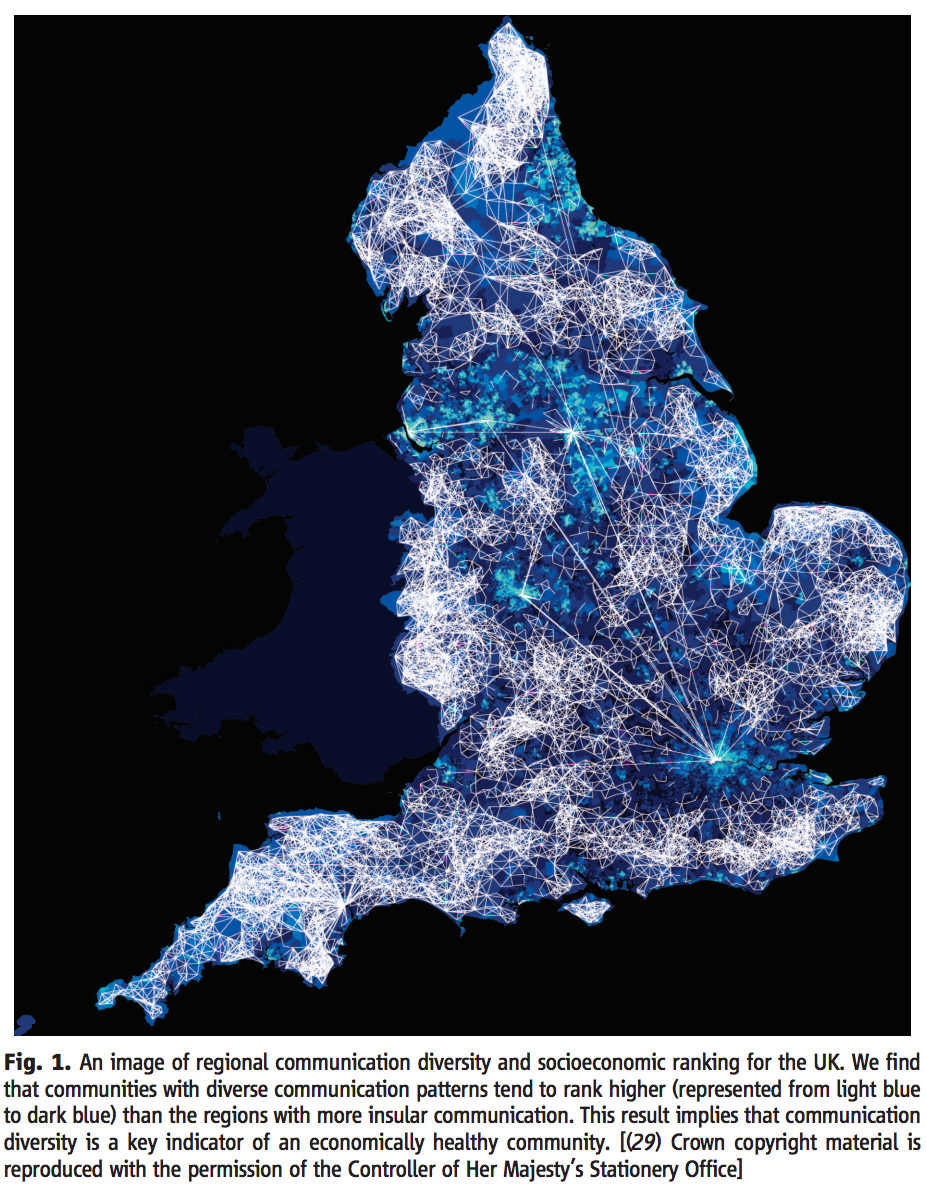
\includegraphics[width=0.50\textwidth]{figures/eagle_et_al.png}
\end{center}

\vf
\tiny{\url{https://science.sciencemag.org/content/328/5981/1029}}

\end{frame}

\begin{frame}{What is digital trace data?}

\begin{center}
	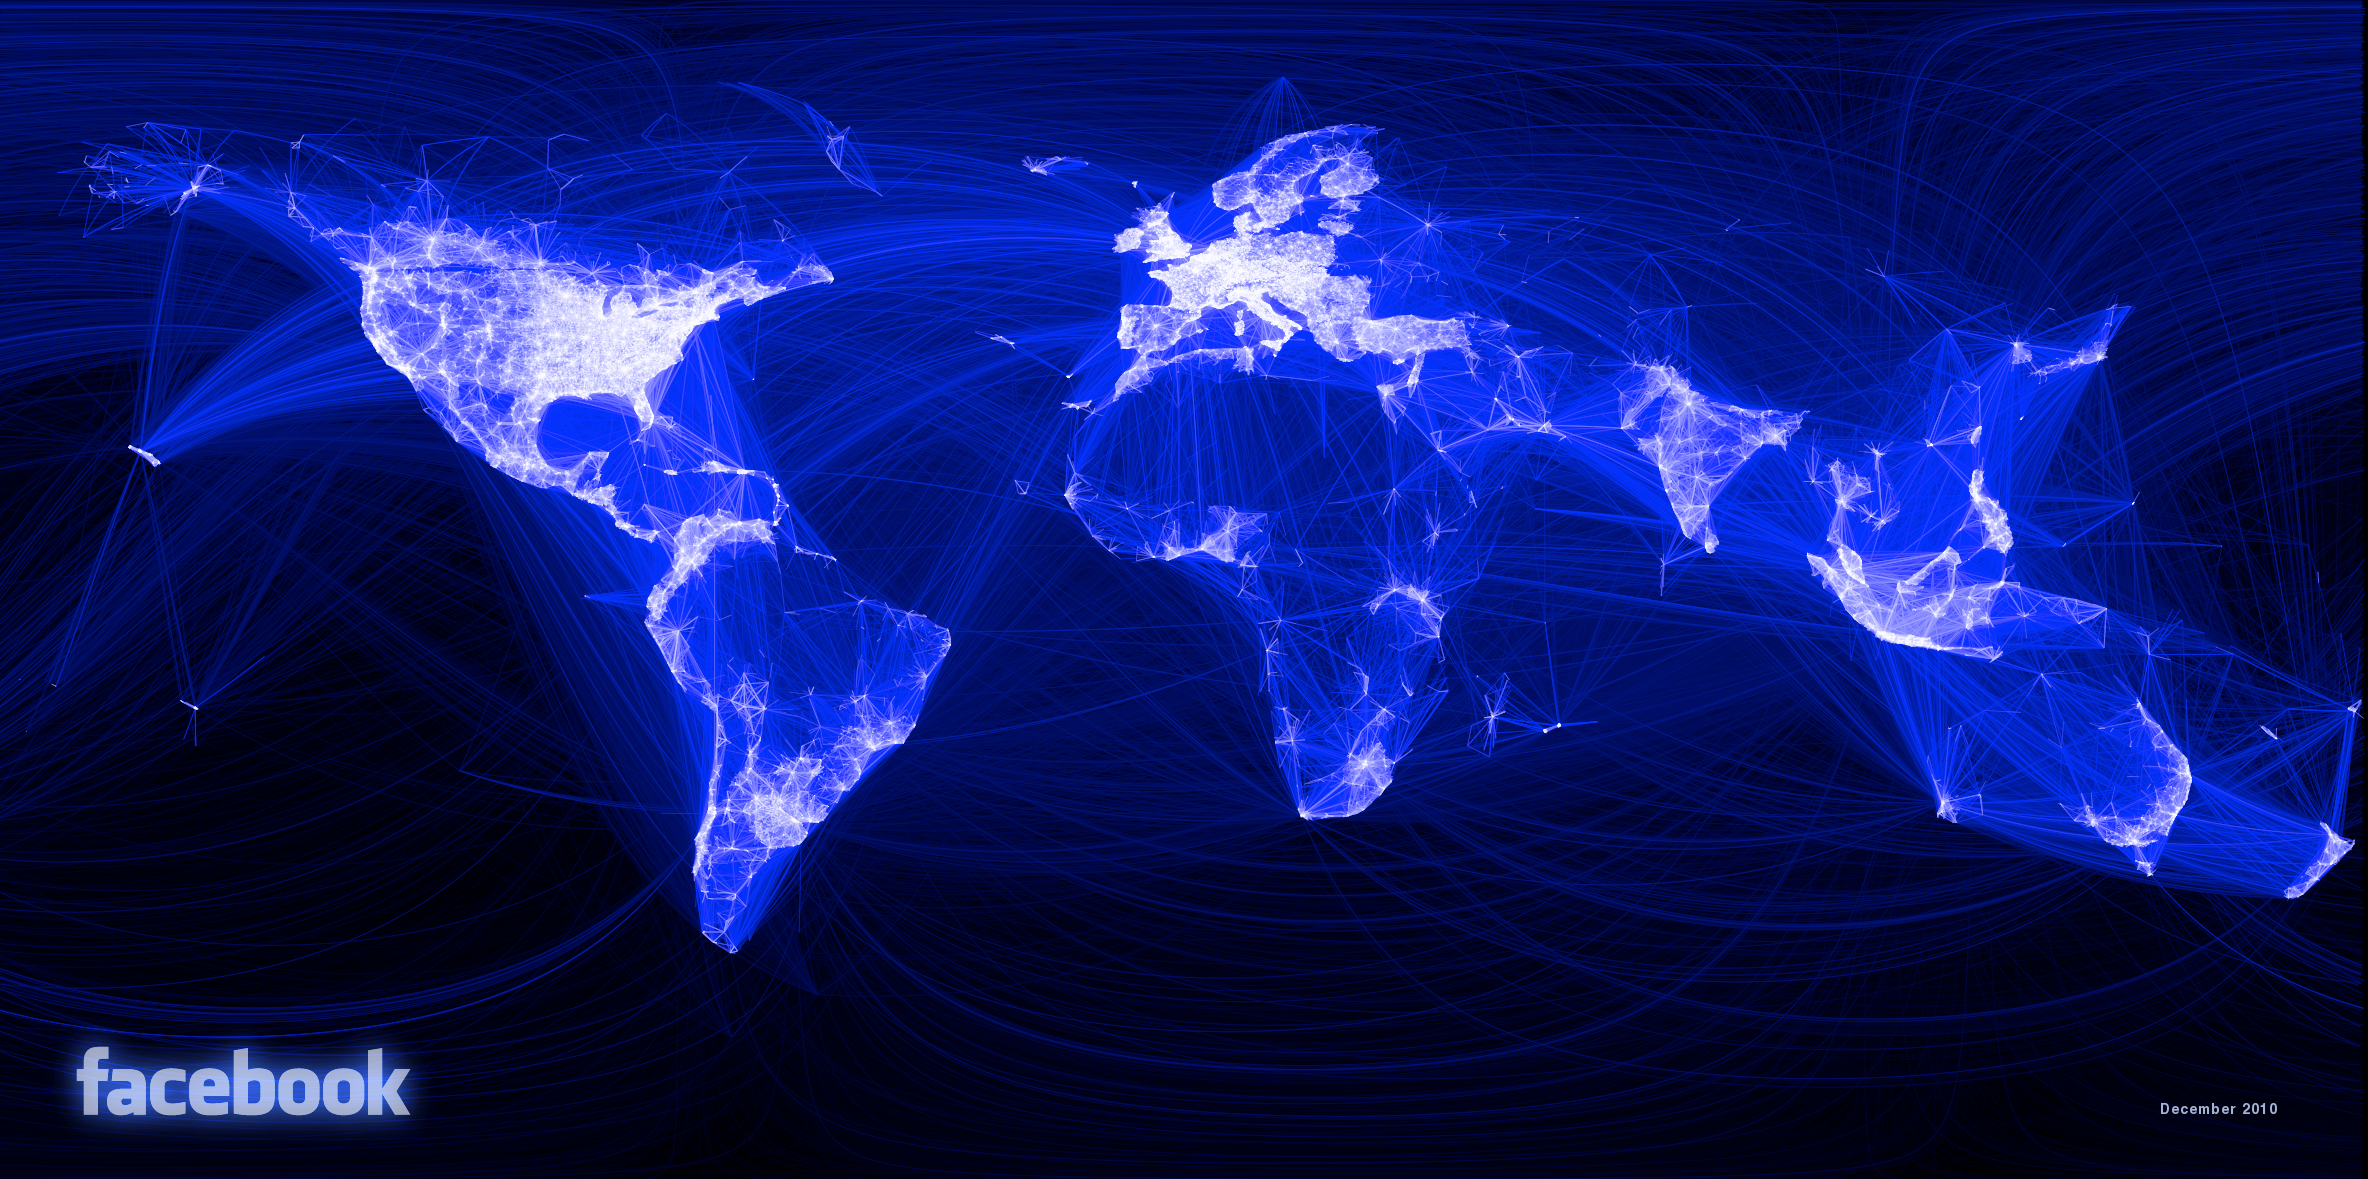
\includegraphics[width=1\textwidth]{figures/facebook_map.png}
\end{center}

\vf
\tiny{\url{https://www.facebook.com/notes/facebook-engineering/visualizing-friendships/469716398919}}

\end{frame}

\begin{frame}{What is digital trace data?}


\begin{center}
	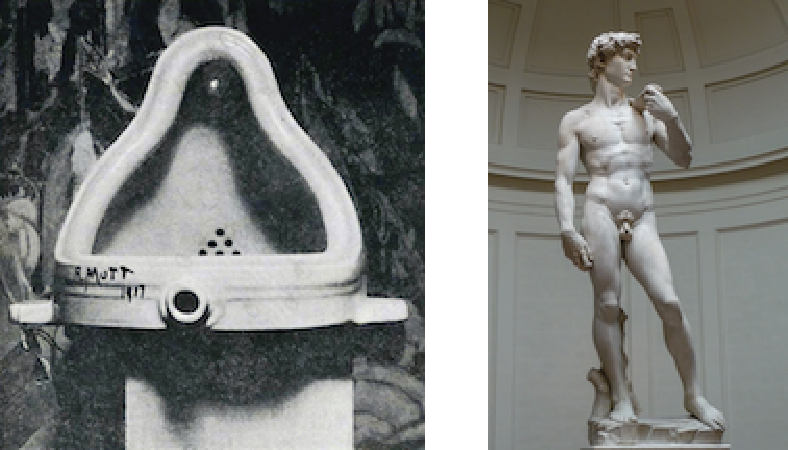
\includegraphics[width=0.9\textwidth]{figures/readymade.png}
\end{center}

\end{frame}

\section{Strengths of digital trace data}


\begin{frame}{Big}

\begin{center}
	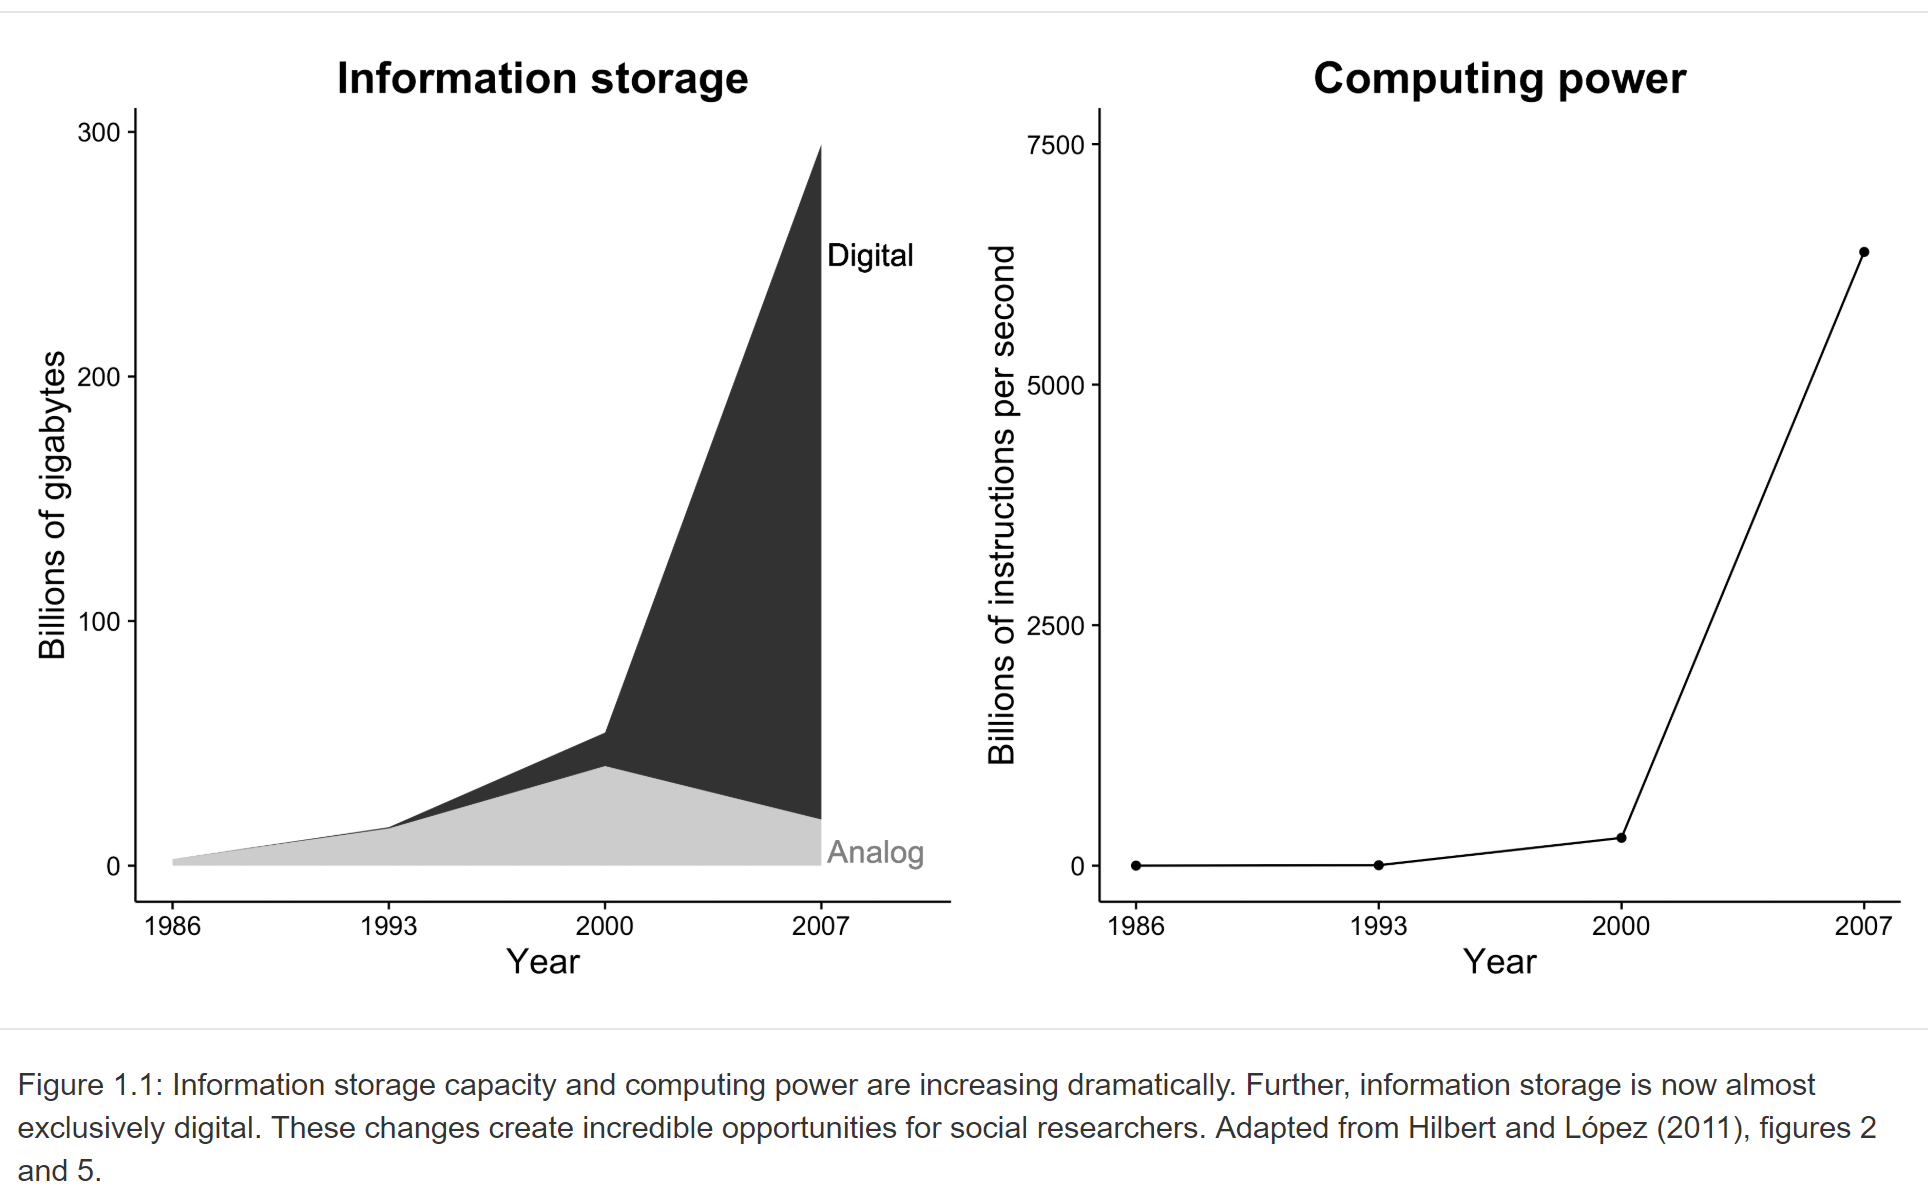
\includegraphics[width=0.95\textwidth]{figures/big_data.png}
\end{center}

\vf
\tiny{\url{https://www.bitbybitbook.com/en/1st-ed/introduction/digital-age/}}
\end{frame}


\begin{frame}{Always on}

\begin{center}
	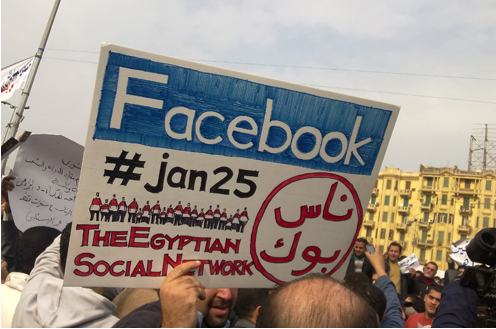
\includegraphics[width=0.95\textwidth]{figures/egypt-arab-spring-facebook-twitter.png}
\end{center}

\vf
\tiny{\url{https://en.wikipedia.org/wiki/Egyptian_revolution_of_2011}}

\end{frame}

\begin{frame}{Non-reactive}

\begin{center}
	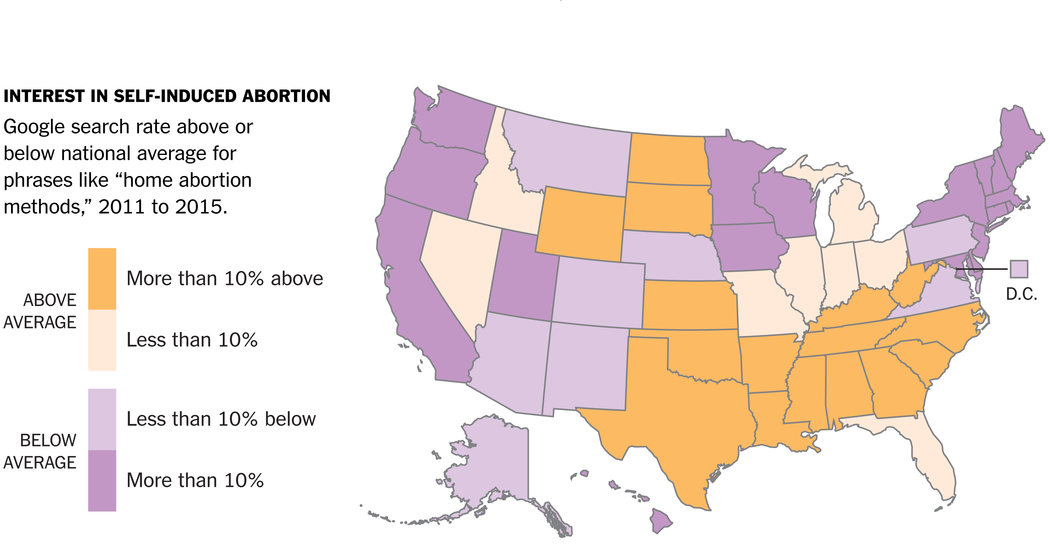
\includegraphics[width=0.95\textwidth]{figures/abortions-at-clinics-or-somewhere-else-1457138970171-facebookJumbo.png}
\end{center}

\vf
\tiny{\url{https://www.nytimes.com/2016/03/06/opinion/sunday/the-return-of-the-diy-abortion.html}}

\end{frame}

\begin{frame}{Captures social relationships}

\begin{center}
	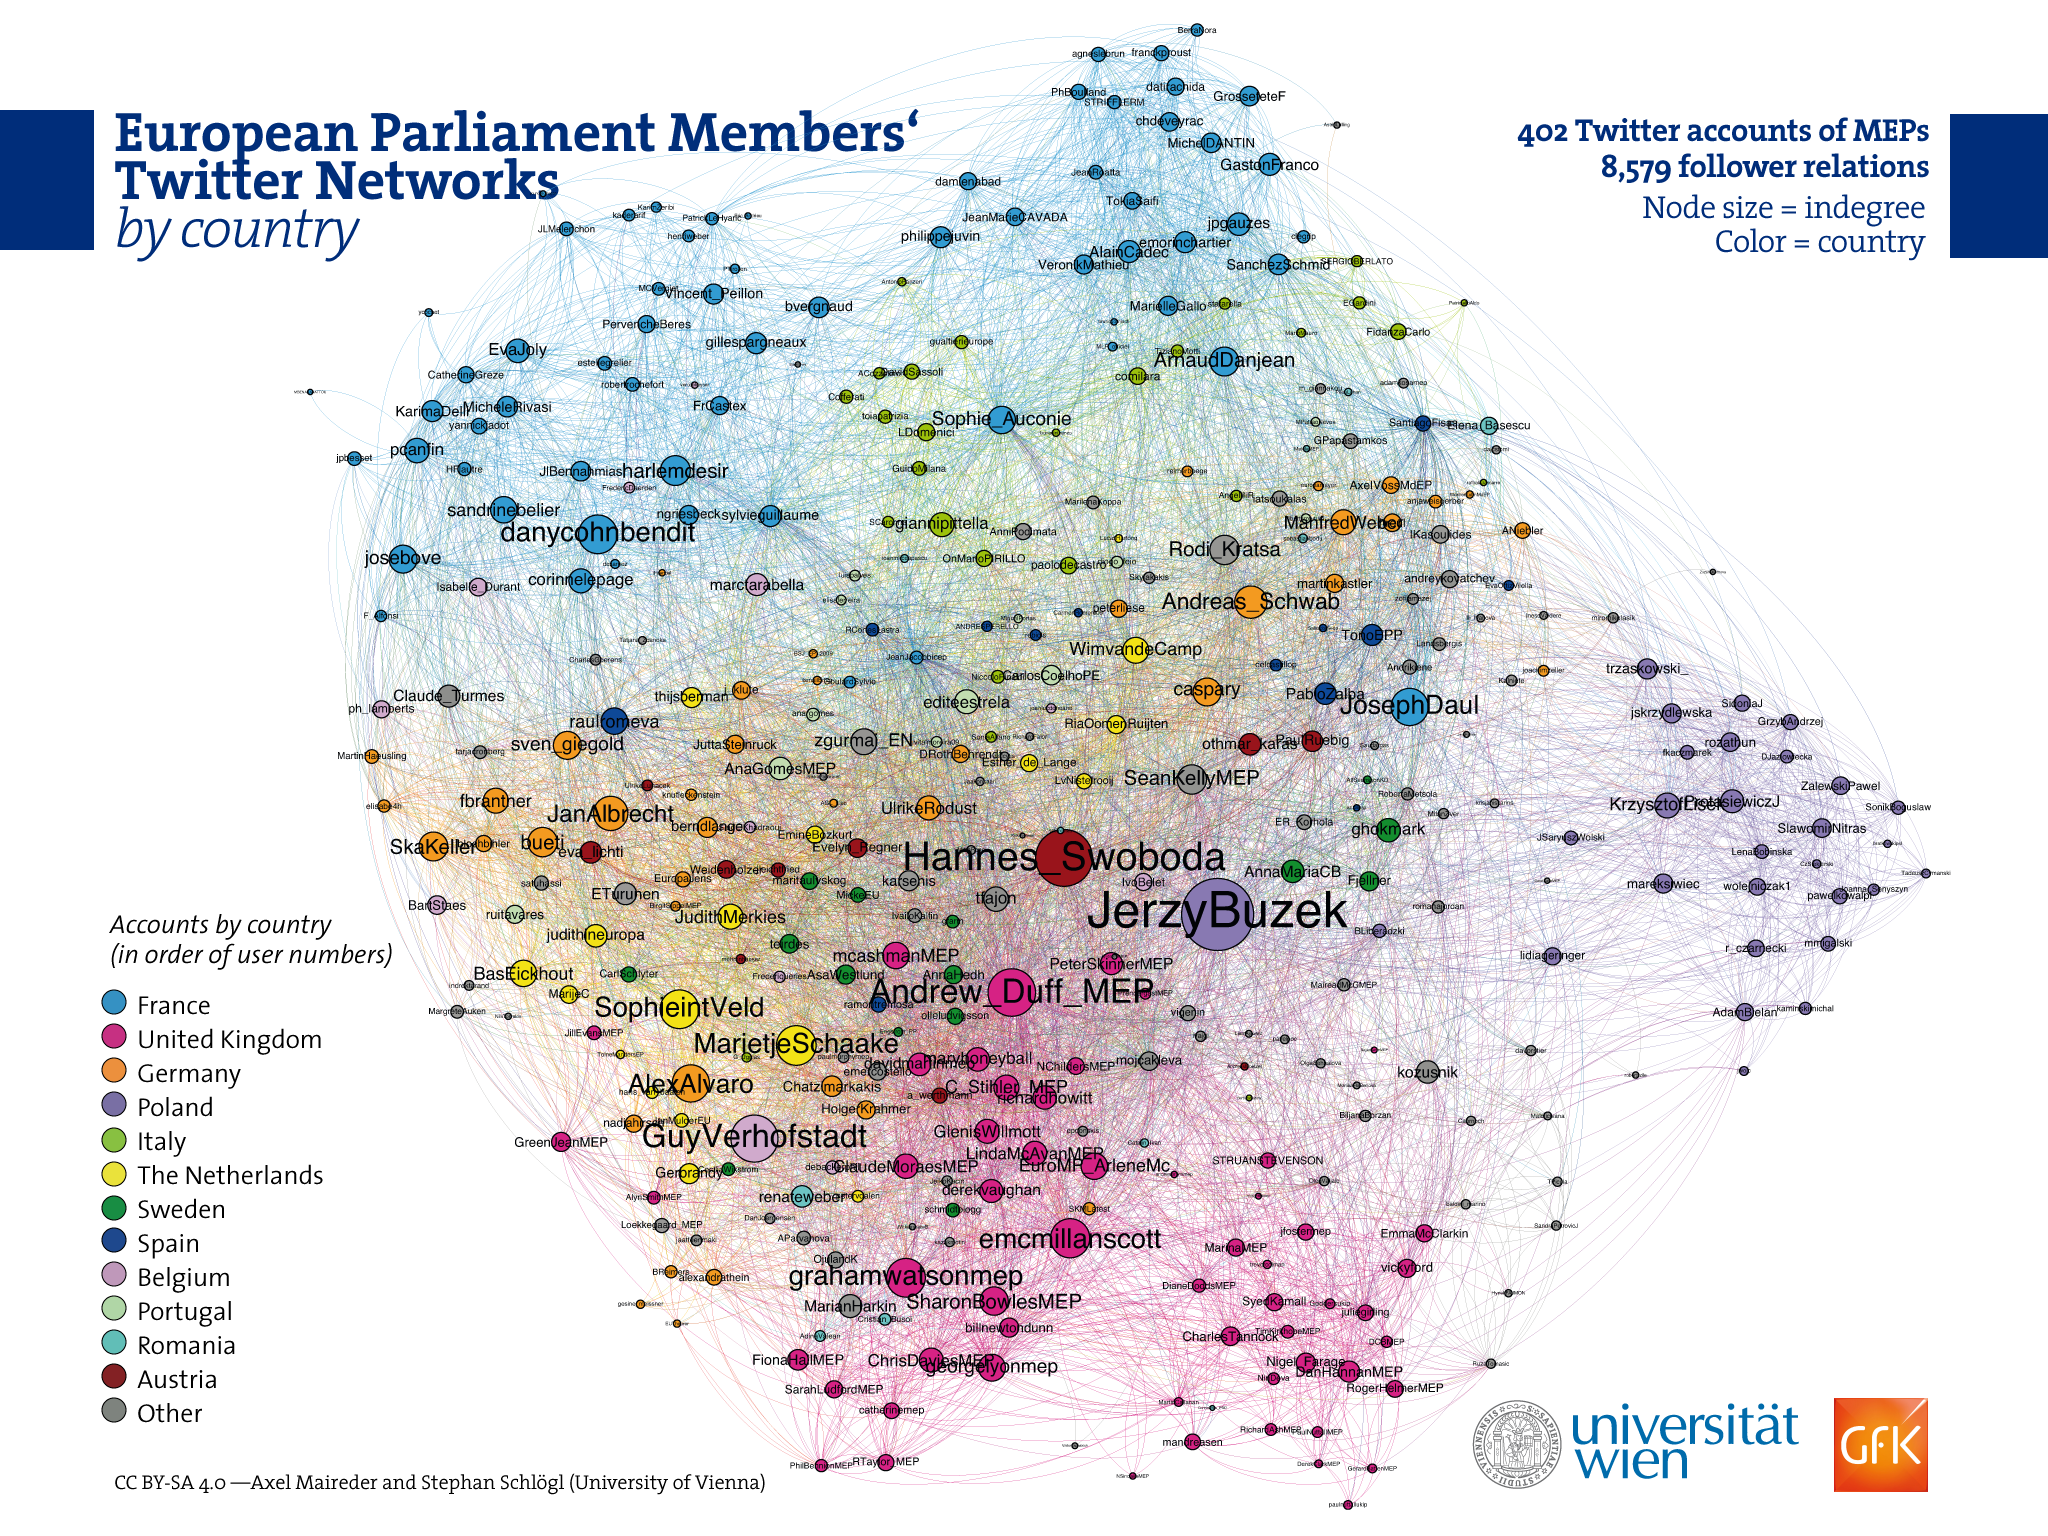
\includegraphics[width=0.8\textwidth]{figures/european_networks.png}
\end{center}

\vf
\tiny{\url{https://homepage.univie.ac.at/axel.maireder/php/wordpress/wp-content/MEPnetwork_country.png}}

\end{frame}

\section{Weaknesses of digital trace data}

\begin{frame}{Incomplete}

\begin{center}
	
\includegraphics[width=0.9\textwidth]{figures/nocomment.jpg}
\end{center}

\end{frame}



\begin{frame}{Inaccessible}

\begin{center}
	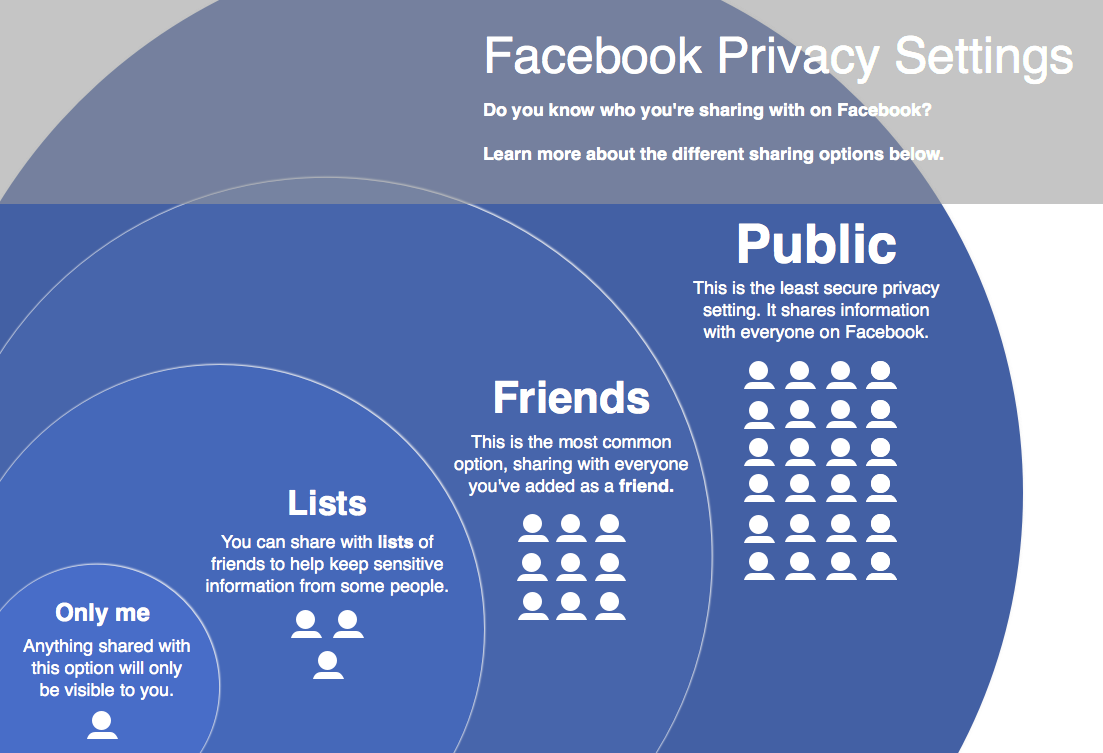
\includegraphics[width=0.9\textwidth]{figures/2014_under_infographic.png}
\end{center}

\end{frame}

\begin{frame}{Non-representative}

\begin{center}
	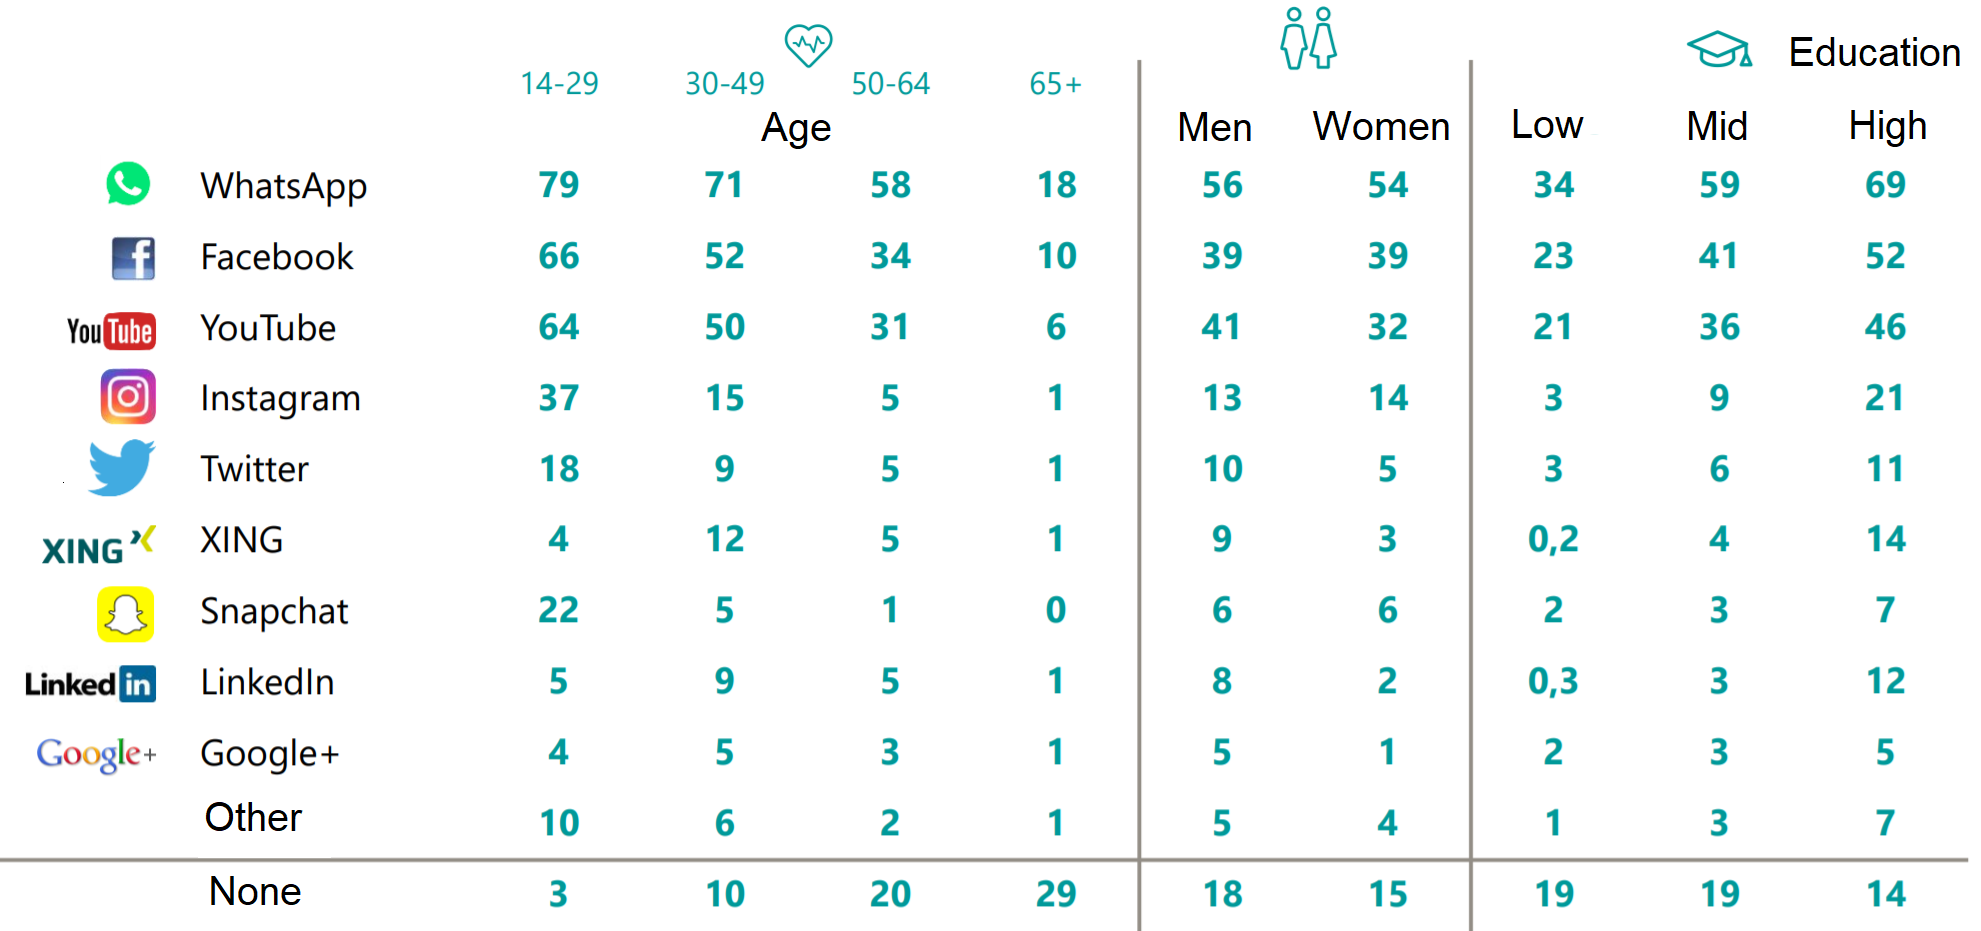
\includegraphics[width=1\textwidth]{figures/nrw_d21_socialmedia.png}
\end{center}

\vf
\tiny{\url{https://initiatived21.de/pm-sonderstudie-nrw/}}

\end{frame}

\begin{frame}{Drifting}

\begin{center}
	
\includegraphics[width=0.7\textwidth]{figures/myspace_2012_original_logo.png}
	\\
	
\includegraphics[width=0.7\textwidth]{figures/studivz_logo.png}
\end{center}

\end{frame}

\begin{frame}{Algorithmically confounded}

\begin{center}
	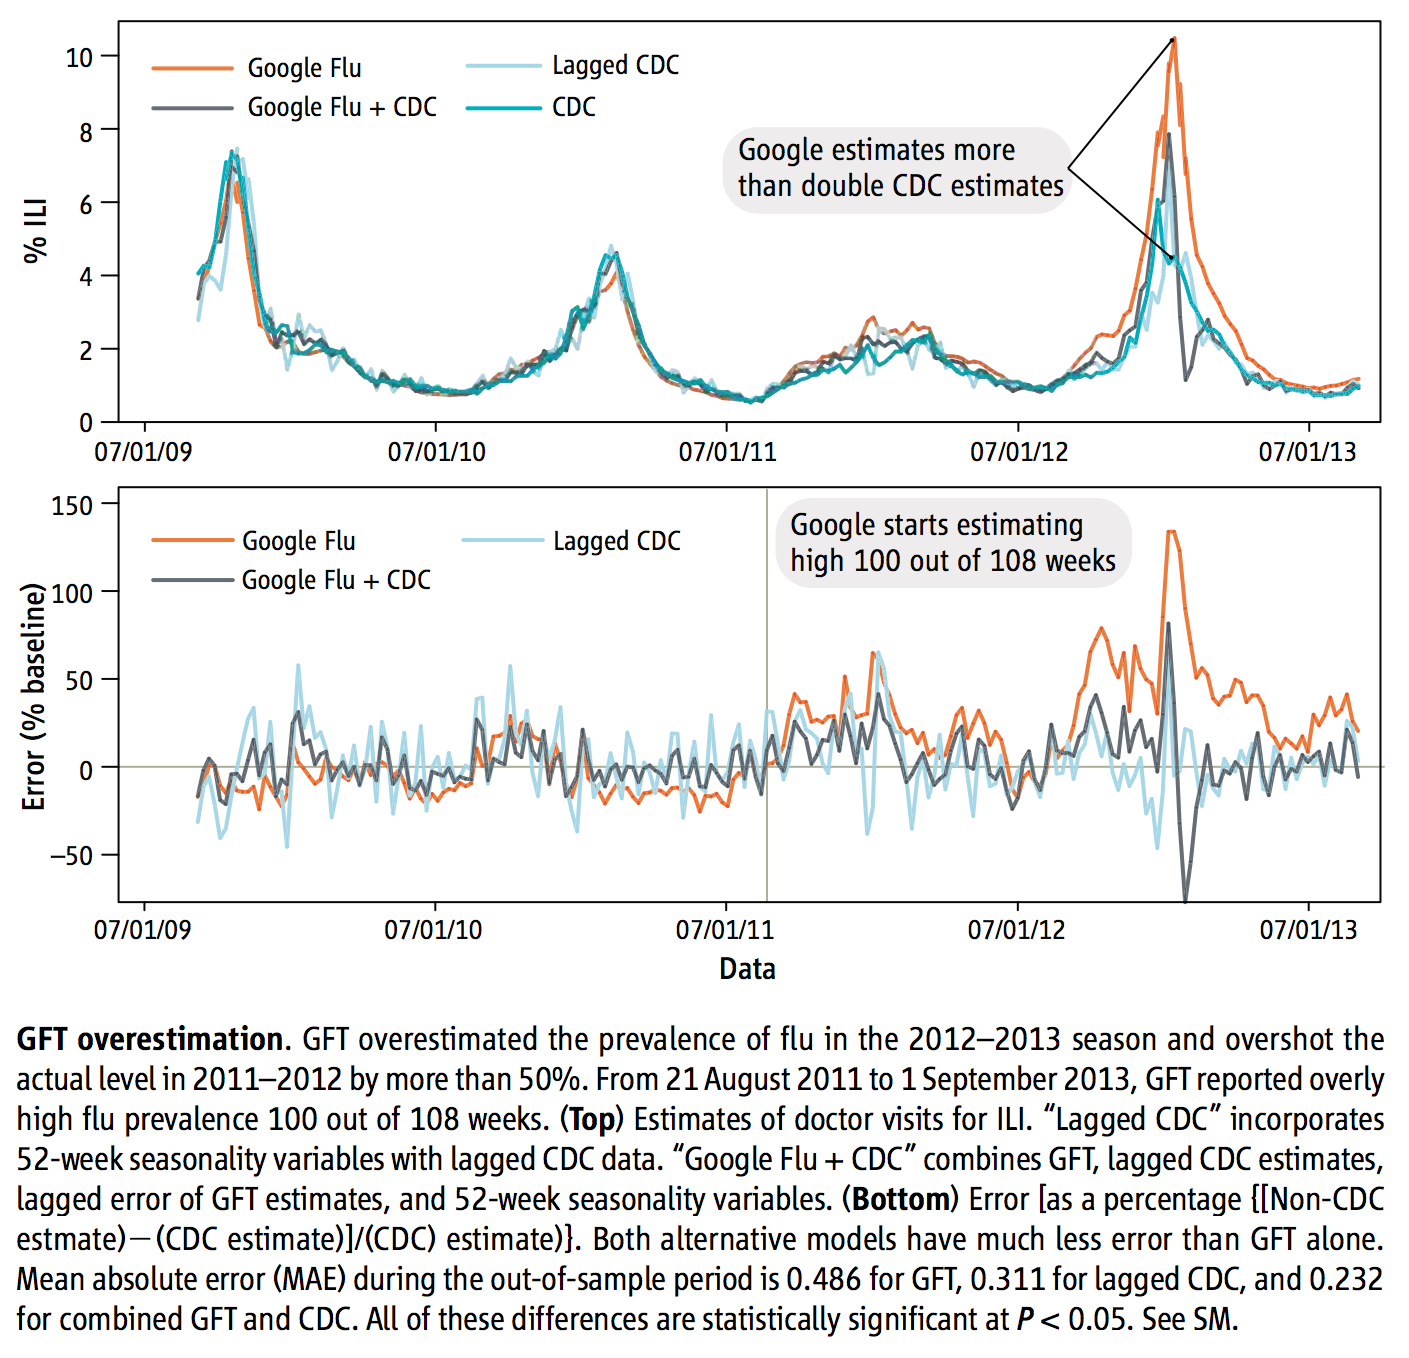
\includegraphics[width=0.65\textwidth]{figures/google_flu.png}

\end{center}
\vf
\tiny{\url{https://dx.doi.org/10.1126/science.1248506}}


\end{frame}

\begin{frame}{Unstructured}

\begin{center}
	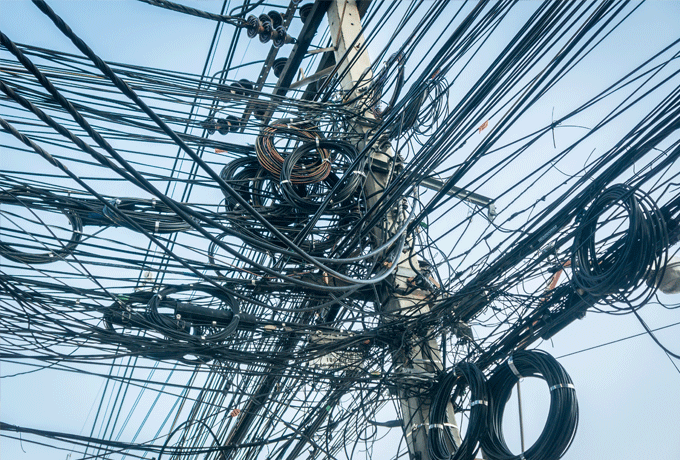
\includegraphics[width=0.8\textwidth]{figures/The-Dirty-Little-Secret-of-Big-Data.png}
	
\end{center}

\end{frame}

\begin{frame}{Sensitive}

\begin{center}
	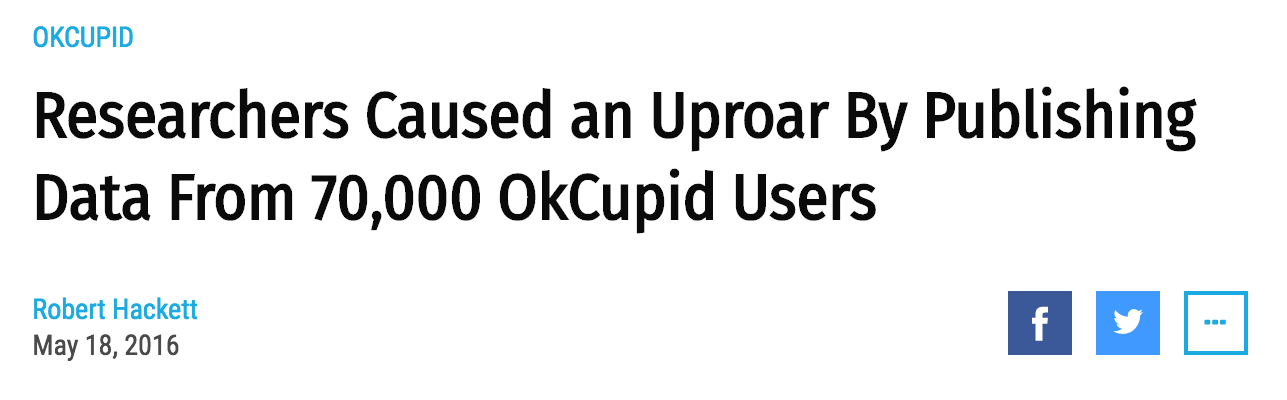
\includegraphics[width=0.9\textwidth]{figures/ok_cupid.png}
	
\end{center}
\vf
\tiny{\url{https://fortune.com/2016/05/18/okcupid-data-research/}}


\end{frame}


\begin{frame}{Positivity bias}

\begin{center}
	
\includegraphics[width=0.9\textwidth]{figures/facebook_positivity_bias.png}
	
\end{center}

\end{frame}


\begin{frame}{The future of digital trace data}

\begin{center}
	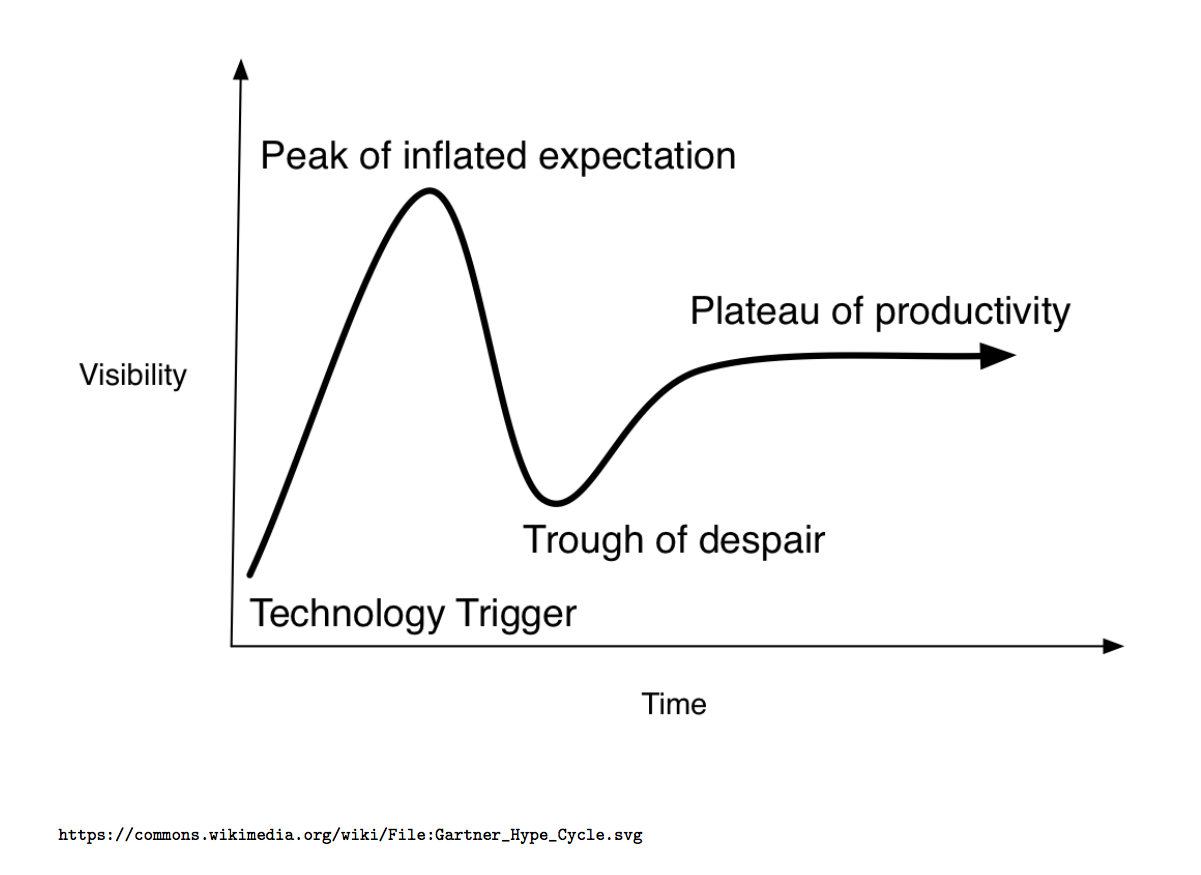
\includegraphics[width=0.9\textwidth]{figures/expectations.png}
	
\end{center}

\end{frame}



\begin{frame}[standout]

\begin{center}
	\LARGE
	Questions?
\end{center}

\end{frame}





\end{document}



